\chapter{Capturas de pantalla}
En este capítulo puede mostrar capturas del sistema para que quede registro del avance del producto. Esta sección es opcional.
\section{Capturas de la funcionalidad X}
Recuerde poner un texto introductorio breve para cada sección.
\vspace{2cm}
\begin{figure}[H]
  \centering
    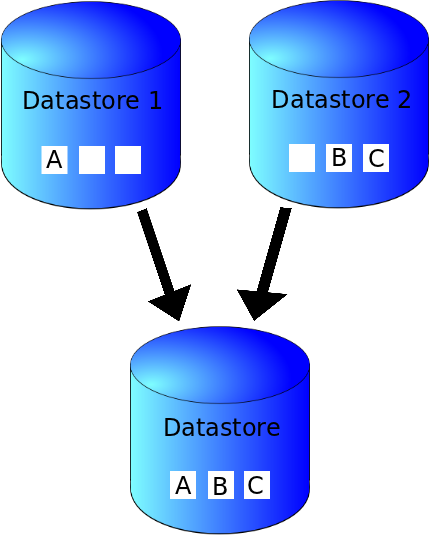
\includegraphics[height= 11cm, width=17cm]{project/images/data-sync}
\end{figure}
\newpage
\begin{figure}[H]
  \centering
    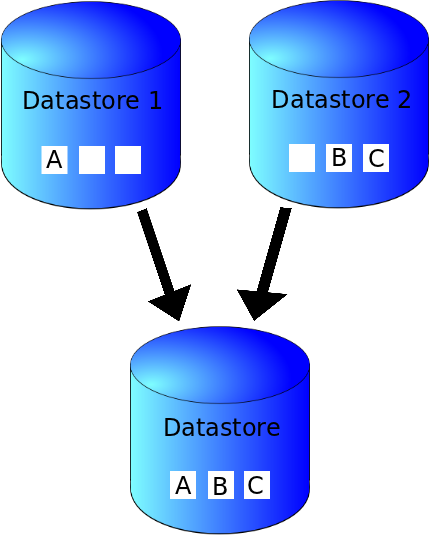
\includegraphics[height= 11cm, width=17cm]{project/images/data-sync}
\end{figure}
\vspace{1cm}

\section{Capturas de la funcionalidad Y}
No olvide referenciar las imágenes en el texto usando \emph{label} y \emph{ref}.

\begin{figure}[H]
  \centering
    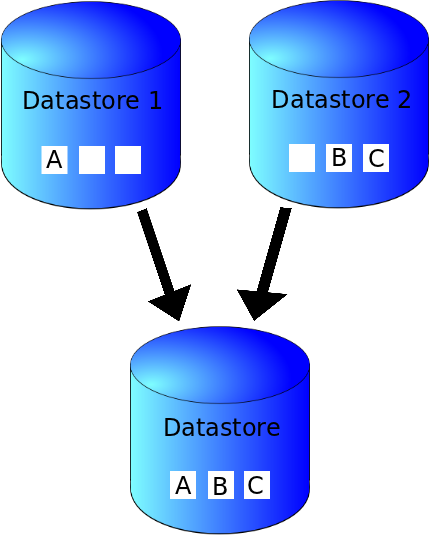
\includegraphics[height= 11cm, width=17cm]{project/images/data-sync}
\end{figure}